\documentclass[11pt,a4paper]{article}

\usepackage[utf8]{inputenc}
\usepackage[T1]{fontenc}
\usepackage{lmodern}
\usepackage[a4paper,margin=2.5cm]{geometry}
\usepackage{graphicx}
\usepackage{amsmath,amssymb}
\usepackage{booktabs}
\usepackage{caption}
\usepackage{subcaption}
\usepackage{float}
\usepackage[hidelinks]{hyperref}
\usepackage{fancyhdr}
\usepackage{xcolor}

\graphicspath{{../figures/}}
\captionsetup{font=small,labelfont=bf}

\pagestyle{fancy}
\fancyhf{}
\lhead{\small Computer Methods in Combustion}
\rhead{\small MKWS 2026}
\cfoot{\thepage}
\renewcommand{\headrulewidth}{0.4pt}

\newcommand{\dme}{\mbox{CH\textsubscript{3}OCH\textsubscript{3}}}

\title{\vspace{-1.0cm}\textbf{Two-Stage Autoignition and Negative Temperature
Coefficient (NTC) Behaviour of Dimethyl Ether (DME)/Air Mixtures}\\[0.3cm]
\large A Homogeneous-Reactor Kinetic Study in Cantera}

\author{\textbf{Grzegorz Wasilczuk} \quad (index no.\ 333514)\\[0.25cm]
Course project --- \emph{Metody Komputerowe w Spalaniu} (MKWS)\\
Warsaw University of Technology, Faculty of Power and Aeronautical Engineering}
\date{June 2026}

\begin{document}
\maketitle
\thispagestyle{fancy}

\begin{abstract}
\noindent The low-temperature autoignition of dimethyl ether (DME, \dme) in air
is studied numerically with the open-source chemical-kinetics library
\textsc{Cantera}. A zero-dimensional, adiabatic, constant-pressure homogeneous
reactor is used to compute ignition delay times (IDT) over the temperature range
625--1300 K, at pressures of 10, 20 and 40 bar and equivalence ratios of 0.5, 1.0
and 2.0, with the hierarchically validated NUI Galway 2015 reaction mechanism
(1268 species, 5336 reactions), which contains the complete low-temperature DME
sub-model. The simulations reproduce the characteristic \emph{negative
temperature coefficient} (NTC) region, in which the ignition delay paradoxically
increases with temperature, and the associated two-stage (cool-flame) ignition.
The strength of the NTC behaviour weakens and shifts to higher temperature as
pressure rises, while the ignition delay decreases monotonically with both
pressure and equivalence ratio. The cool-flame chemistry is traced to the
build-up and decomposition of the CH\textsubscript{3}OCH\textsubscript{2}O\textsubscript{2}
peroxy radical and of formaldehyde.
\end{abstract}

\section{Introduction}
Dimethyl ether is the simplest ether and an attractive alternative fuel: it can
be produced from biomass, natural gas or captured CO\textsubscript{2}, it has a
high cetane number ($\approx$ 55--60), and its soot-free combustion makes it a
candidate for compression-ignition (diesel) and homogeneous-charge
compression-ignition (HCCI) engines. Because DME ignites through the same
low-temperature radical chemistry as large alkanes, it is also a key benchmark
fuel for validating detailed kinetic mechanisms.

A defining feature of such fuels is the \textbf{negative temperature coefficient
(NTC)} of the ignition delay: over an intermediate temperature window (roughly
750--1000 K) the overall reactivity decreases as the temperature rises, so that
the mixture ignites \emph{more slowly} when it is hotter. The NTC region is
accompanied by \textbf{two-stage ignition}, in which a weak, low-temperature heat
release --- the \emph{cool flame} --- precedes the main ignition event. These
phenomena directly control engine knock, HCCI combustion phasing and the
operability limits of advanced low-temperature combustion engines, which is why
their accurate prediction is of practical importance.

The aim of this project is to reproduce and analyse the NTC behaviour and the
two-stage autoignition of DME/air mixtures using a detailed chemical-kinetics
model, and to quantify how the ignition delay and the strength of the NTC region
depend on temperature, pressure and equivalence ratio. All computations are
carried out with \textsc{Cantera} in Python; the full source code accompanies
this report.

\section{Literature review}
The low-temperature oxidation of DME was characterised experimentally and
kinetically by Curran et al.~\cite{curran2000}, who established the degenerate
chain-branching pathway responsible for cool flames. The comprehensive mechanism
of Zhao et al.~\cite{zhao2008} (55 species, 290 reactions) became the standard
reference model for DME and reproduces shock-tube ignition delays, flow-reactor
speciation and laminar flame speeds. Burke et al.~\cite{burke2015} extended the
validation to high pressures (up to 110 bar) for methane, DME and their blends,
and their NUI Galway model forms the basis of the AramcoMech family of
hierarchically constructed mechanisms~\cite{metcalfe2013}. Reduced models
suitable for CFD, such as the 30-species skeletal mechanism of Bhagatwala et
al.~\cite{bhagatwala2015} and the reduced model of Pan et al.~\cite{pan2015},
retain the low-temperature chemistry required to capture the NTC region.

The chemical origin of the NTC behaviour is now well
understood~\cite{westbrook2000,griffiths1995}. At low temperature the fuel
radical R$^{\bullet}$ (here CH\textsubscript{3}OCH\textsubscript{2}$^{\bullet}$)
adds molecular oxygen to form a peroxy radical RO\textsubscript{2}, which
isomerises to a hydroperoxyalkyl radical $^{\bullet}$QOOH and, after a second
O\textsubscript{2} addition, leads to chain branching through ketohydroperoxide
decomposition. As the temperature rises, the
RO\textsubscript{2} $\rightleftharpoons$ R + O\textsubscript{2} equilibrium
shifts back towards the reactants, suppressing this branching pathway; the system
must then wait for the slower intermediate-temperature
H\textsubscript{2}O\textsubscript{2} chemistry to take over, which is the
microscopic cause of the increase in ignition delay with temperature.

\section{Numerical model}
\subsection{Software and chemistry}
All computations use \textsc{Cantera}~3.2 with the NUI Galway 2015 hierarchical
mechanism (the \texttt{n-hexane-NUIG-2015} model distributed with Cantera as
example data), comprising 1268 species and 5336 elementary reactions and built on
the comprehensively validated AramcoMech C\textsubscript{0}--C\textsubscript{2}
core~\cite{metcalfe2013}. Although developed for the hexane isomers, the model
contains the complete low-temperature DME sub-mechanism (the
CH\textsubscript{3}OCH\textsubscript{2}O\textsubscript{2} /
CH\textsubscript{3}OCH\textsubscript{2}O\textsubscript{2}H / ketohydroperoxide
pathway); DME (\dme) is therefore taken directly as the fuel. Air is modelled as
O\textsubscript{2}:N\textsubscript{2} = 1:3.76.

\subsection{Reactor model and governing equations}
Autoignition is modelled with a homogeneous (zero-dimensional), adiabatic,
constant-pressure batch reactor, which represents an isolated fluid element of a
premixed charge. For a closed adiabatic system at constant pressure the governing
equations solved by Cantera are the species and energy balances
\begin{equation}
\frac{dY_k}{dt} = \frac{\dot{\omega}_k W_k}{\rho}, \qquad
c_p\,\frac{dT}{dt} = -\frac{1}{\rho}\sum_k h_k\,\dot{\omega}_k W_k ,
\end{equation}
where $Y_k$, $W_k$, $h_k$ and $\dot{\omega}_k$ are the mass fraction, molar mass,
specific enthalpy and net molar production rate of species $k$, $\rho$ is the
density, $c_p$ the mixture specific heat and $T$ the temperature. The resulting
stiff system of ODEs is integrated with the CVODES solver (absolute tolerance
$10^{-15}$, relative tolerance $10^{-6}$).

\subsection{Ignition-delay definition and two-stage detection}
The total ignition delay time (IDT) is defined as the instant of maximum
temperature-rise rate, i.e.\ the time at which $dT/dt$ reaches its global maximum.
The first-stage (cool-flame) delay is identified as the first significant local
maximum of $dT/dt$ preceding the main event; a cool flame is reported only when
this early peak is clearly separated from the main ignition. This dual criterion
extracts both stages of a two-stage ignition automatically from a single reactor
integration. Initial temperatures were varied from 625 to 1300 K (28 points);
the pressure was set to 10, 20 and 40 bar at stoichiometric conditions, and the
equivalence ratio to $\phi = 0.5, 1.0, 2.0$ at 20 bar --- in total 5 temperature
sweeps ($\approx$ 140 reactor simulations) plus three time-resolved ignition
histories.

\section{Results and discussion}
\subsection{NTC region and the effects of pressure and equivalence ratio}
Figure~\ref{fig:scurve} shows the computed ignition delay of DME/air as a
function of inverse temperature. All curves display the classic S-shape: a
high-temperature branch (left), the NTC region in the middle, where the delay
increases with temperature, and a low-temperature branch (right). The NTC region
is most pronounced at the lowest pressure (Fig.~\ref{fig:pressure}) and persists
at every equivalence ratio (Fig.~\ref{fig:phi}).

\begin{figure}[H]
  \centering
  \begin{subfigure}{0.49\textwidth}
    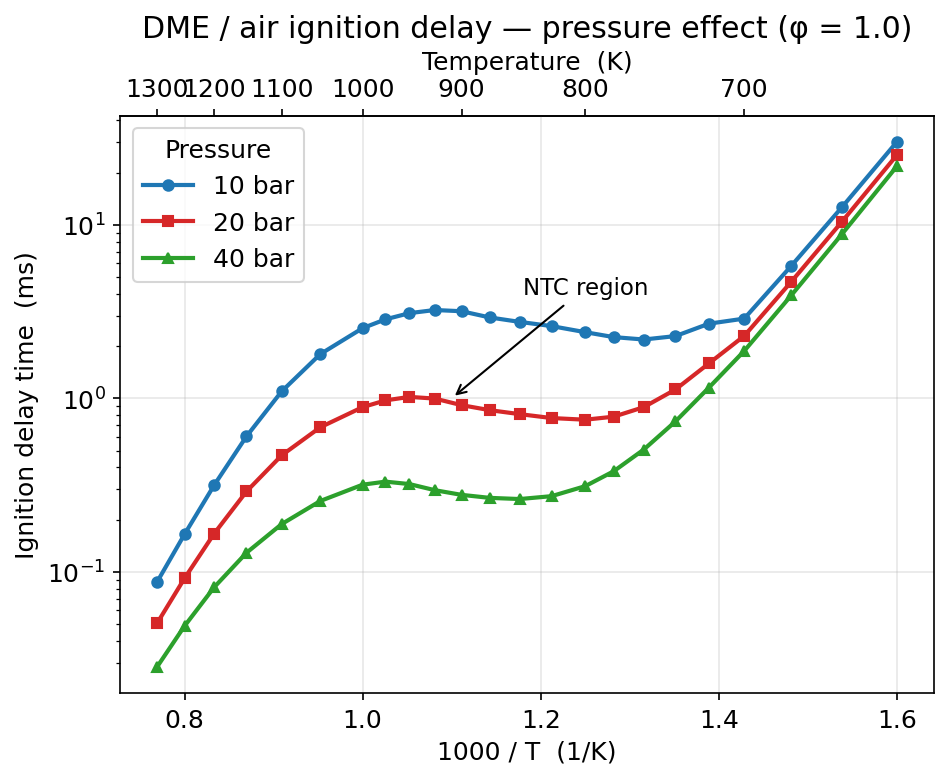
\includegraphics[width=\linewidth]{fig1_pressure_ntc.png}
    \caption{Effect of pressure ($\phi=1.0$).}
    \label{fig:pressure}
  \end{subfigure}\hfill
  \begin{subfigure}{0.49\textwidth}
    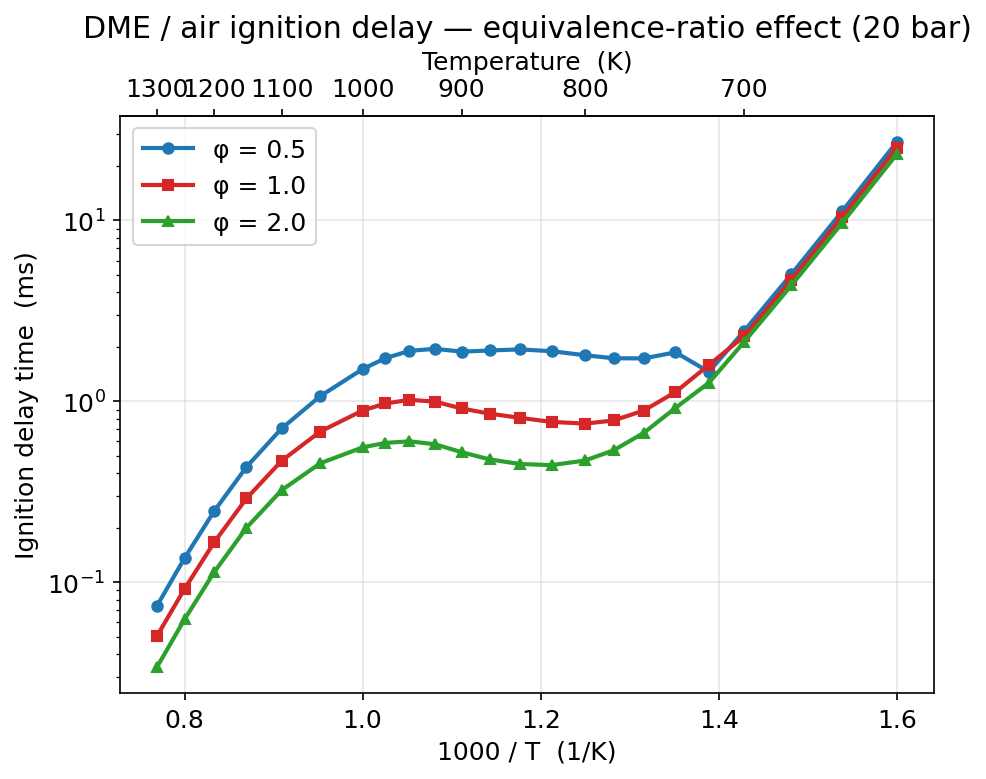
\includegraphics[width=\linewidth]{fig2_equivalence_ratio.png}
    \caption{Effect of equivalence ratio (20 bar).}
    \label{fig:phi}
  \end{subfigure}
  \caption{Ignition delay of DME/air versus inverse temperature. The
  non-monotonic NTC region is visible in every case.}
  \label{fig:scurve}
\end{figure}

Table~\ref{tab:ntc} quantifies the NTC region. As pressure rises from 10 to
40 bar, the whole curve shifts to shorter delays (higher reactivity), the NTC
zone moves to higher temperature (valley from 760 to 850 K), and the strength of
the NTC --- the ratio of the local-maximum to the local-minimum delay --- weakens
from 1.48 to 1.26. This is the expected behaviour: higher pressure favours the
chain-branching O\textsubscript{2} addition steps and broadens the temperature
window over which they remain active. Increasing the equivalence ratio shortens
the ignition delay throughout the high-temperature and NTC regions --- at 1000 K
the delay falls from 1.51 ms ($\phi=0.5$) to 0.89 ms ($\phi=1.0$) and 0.56 ms
($\phi=2.0$) --- because a higher fuel concentration accelerates the
rate-limiting fuel\,+\,OH and RO\textsubscript{2} isomerisation steps. On the
low-temperature branch the three $\phi$ curves converge, indicating that there
the delay is governed by the intrinsic low-temperature chain chemistry rather
than by the amount of fuel present.

\begin{table}[H]
\centering
\caption{Location and strength of the NTC region (stoichiometric DME/air).}
\label{tab:ntc}
\begin{tabular}{ccccc}
\toprule
Pressure (bar) & Valley $T$ (K) & Valley IDT (ms) & Peak $T$ (K) & Peak/valley \\
\midrule
10 & 760 & 2.18 & 925 & 1.48 \\
20 & 800 & 0.75 & 950 & 1.35 \\
40 & 850 & 0.26 & 975 & 1.26 \\
\bottomrule
\end{tabular}
\end{table}

\subsection{Two-stage (cool-flame) ignition and low-temperature chemistry}
Figure~\ref{fig:hist} presents the time history of a representative case inside
the NTC window ($T_0 = 850$ K, 20 bar, $\phi = 1.0$). The temperature trace
exhibits two distinct rises: a small step of about 100 K at $\approx$ 0.15 ms ---
the cool flame --- followed by a thermal-runaway main ignition at $\approx$
0.81 ms. The lower panel, showing $dT/dt$ on a logarithmic scale, makes the two
heat-release pulses unambiguous. The cool flame partially consumes the fuel and
raises the temperature into the range where the low-temperature branching becomes
inefficient, introducing the induction period that separates the two stages ---
the very mechanism that produces the NTC behaviour of
Figure~\ref{fig:scurve}.

\begin{figure}[H]
  \centering
  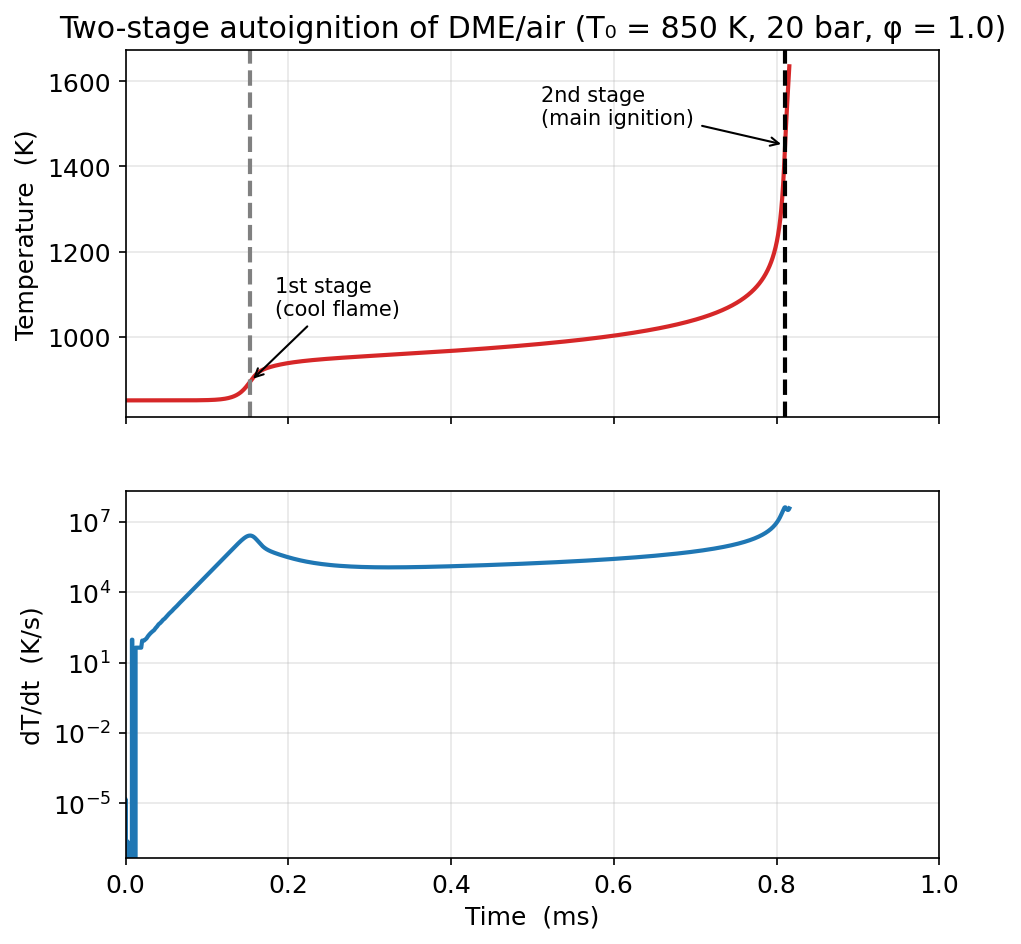
\includegraphics[width=0.6\textwidth]{fig3_twostage_history.png}
  \caption{Two-stage autoignition of DME/air (850 K, 20 bar, $\phi=1.0$). Top:
  temperature; bottom: temperature-rise rate. The cool flame precedes the main
  ignition by about 0.65 ms.}
  \label{fig:hist}
\end{figure}

Figure~\ref{fig:species} follows the key species during the same ignition. During
the cool-flame stage the peroxy radical
CH\textsubscript{3}OCH\textsubscript{2}O\textsubscript{2} (scaled $\times$50)
rises and falls in a sharp pulse, while formaldehyde CH\textsubscript{2}O
accumulates --- both are the fingerprints of the RO\textsubscript{2}/QOOH
low-temperature pathway. Only a fraction of the DME is consumed at this stage.
The accumulated intermediates (CH\textsubscript{2}O,
H\textsubscript{2}O\textsubscript{2}) then decompose, the OH ($\times$20) and CO
pools explode, the remaining fuel and O\textsubscript{2} are consumed and the
temperature runs away to the adiabatic flame value --- the main ignition.
Figure~\ref{fig:first} plots the cool-flame delay together with the total delay:
a distinct first stage is detected only inside the NTC window
($\approx$ 720--900 K); the cool-flame delay decreases monotonically with
temperature, whereas the total delay turns over, confirming that it is the
lengthening induction \emph{between} the two stages, not the cool flame itself,
that creates the NTC behaviour.

\begin{figure}[H]
  \centering
  \begin{subfigure}{0.49\textwidth}
    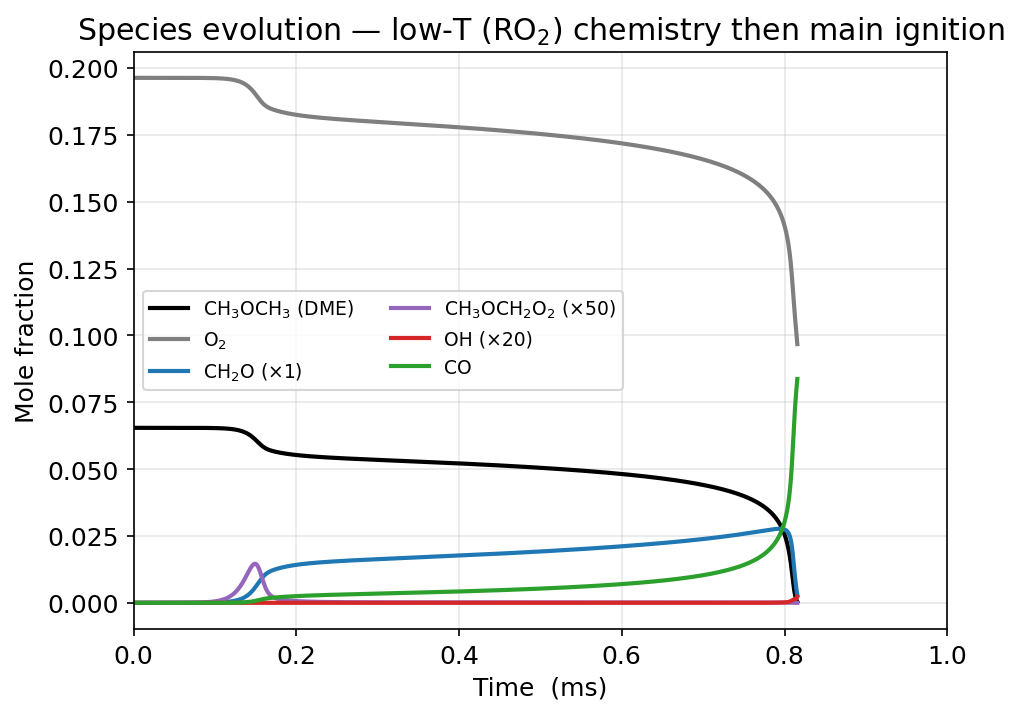
\includegraphics[width=\linewidth]{fig4_species.png}
    \caption{Species evolution.}
    \label{fig:species}
  \end{subfigure}\hfill
  \begin{subfigure}{0.49\textwidth}
    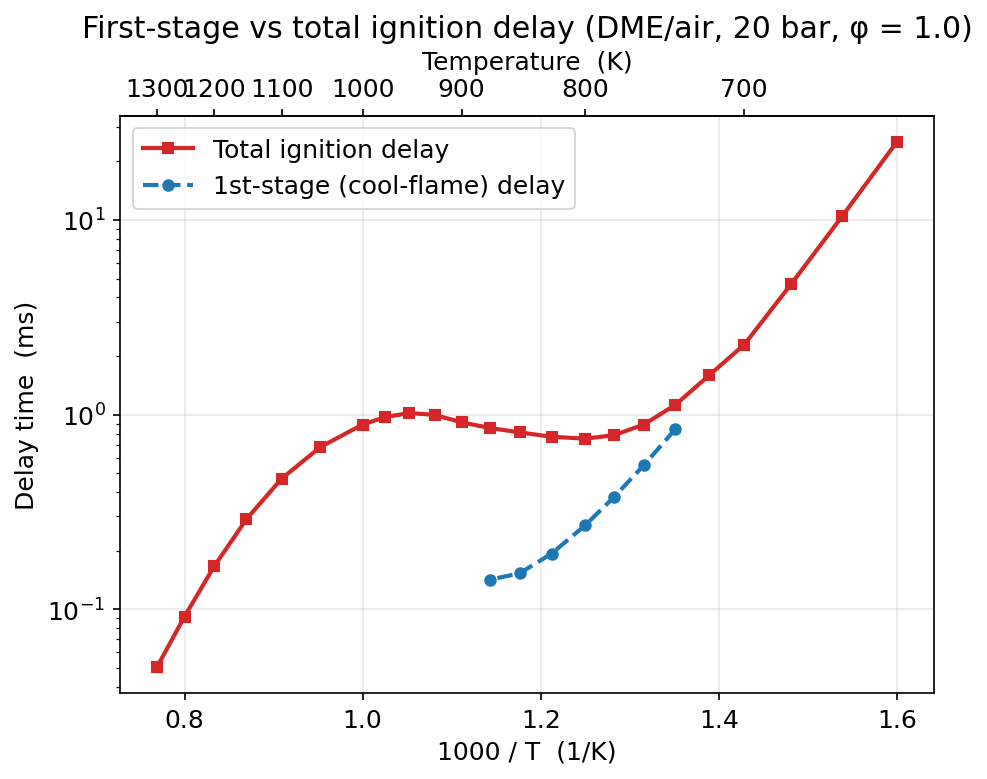
\includegraphics[width=\linewidth]{fig5_first_vs_total.png}
    \caption{First-stage vs.\ total delay.}
    \label{fig:first}
  \end{subfigure}
  \caption{Low-temperature chemistry. Left: mole-fraction history at 850 K,
  20 bar (the CH\textsubscript{3}OCH\textsubscript{2}O\textsubscript{2} pulse and
  CH\textsubscript{2}O build-up mark the cool flame). Right: the cool flame
  appears only inside the NTC window.}
  \label{fig:lowT}
\end{figure}

\section{Conclusions}
A detailed chemical-kinetics study of DME/air autoignition was carried out in
\textsc{Cantera} using a zero-dimensional adiabatic constant-pressure reactor and
the NUI Galway 2015 mechanism. The main findings are:
\begin{enumerate}
  \item The model reproduces the characteristic NTC region of DME, in which the
  ignition delay increases with temperature between roughly 760 and 975 K.
  \item Raising the pressure from 10 to 40 bar shortens the ignition delay,
  shifts the NTC region to higher temperature and weakens it (NTC strength
  falling from 1.48 to 1.26).
  \item Richer mixtures ignite faster; the equivalence ratio has little effect on
  the low-temperature branch, where the intrinsic chain chemistry dominates.
  \item Inside the NTC window the ignition is two-stage: a cool flame, driven by
  the CH\textsubscript{3}OCH\textsubscript{2}O\textsubscript{2} peroxy-radical
  chemistry and formaldehyde build-up, precedes the main ignition. The NTC
  behaviour arises from the lengthening induction period between the two stages
  as the RO\textsubscript{2} branching pathway is progressively shut off with
  rising temperature.
\end{enumerate}
The results are physically consistent and in qualitative agreement with the
published DME literature~\cite{zhao2008,burke2015}, demonstrating that 0-D
homogeneous-reactor modelling in \textsc{Cantera} captures the essential
low-temperature combustion physics relevant to engine knock and HCCI combustion.
The principal modelling limitation is the use of a detailed but generic NUIG
mechanism rather than a dedicated, separately optimised DME model; a
constant-volume reactor and a sensitivity analysis of the controlling
RO\textsubscript{2} reactions would further refine the absolute delay times
without changing the qualitative conclusions.

\begin{thebibliography}{9}
\bibitem{curran2000} H.~J. Curran, S.~L. Fischer, F.~L. Dryer. The reaction
kinetics of dimethyl ether. II: Low-temperature oxidation in flow reactors.
\emph{Int. J. Chem. Kinet.} 32 (2000) 741--759.
\bibitem{zhao2008} Z.~Zhao, M.~Chaos, A.~Kazakov, F.~L. Dryer. Thermal
decomposition reaction and a comprehensive kinetic model of dimethyl ether.
\emph{Int. J. Chem. Kinet.} 40 (2008) 1--18.
\bibitem{burke2015} U.~Burke, K.~P. Somers, P.~O'Toole, et al. An ignition delay
and kinetic modeling study of methane, dimethyl ether, and their mixtures at high
pressures. \emph{Combust. Flame} 162 (2015) 315--330.
\bibitem{pan2015} L.~Pan, S.~Kokjohn, Z.~Huang. Development and validation of a
reduced chemical kinetic model for dimethyl ether combustion. \emph{Fuel} 160
(2015) 165--177.
\bibitem{bhagatwala2015} A.~Bhagatwala, Z.~Luo, H.~Shen, J.~A. Sutton, T.~Lu,
J.~H. Chen. Numerical and experimental investigation of turbulent DME jet flames.
\emph{Proc. Combust. Inst.} 35 (2015) 1157--1166.
\bibitem{westbrook2000} C.~K. Westbrook. Chemical kinetics of hydrocarbon
ignition in practical combustion systems. \emph{Proc. Combust. Inst.} 28 (2000)
1563--1577.
\bibitem{griffiths1995} J.~F. Griffiths. Reduced kinetic models and their
application to practical combustion systems. \emph{Prog. Energy Combust. Sci.} 21
(1995) 25--107.
\bibitem{goodwin2024} D.~G. Goodwin, H.~K. Moffat, I.~Schoegl, R.~L. Speth,
B.~W. Weber. \emph{Cantera: An Object-oriented Software Toolkit for Chemical
Kinetics, Thermodynamics, and Transport Processes}, version 3.2, 2024.
\url{https://www.cantera.org}
\bibitem{metcalfe2013} W.~K. Metcalfe, S.~M. Burke, S.~S. Ahmed, H.~J. Curran. A
hierarchical and comparative kinetic modeling study of
C\textsubscript{1}--C\textsubscript{2} hydrocarbon and oxygenated fuels.
\emph{Int. J. Chem. Kinet.} 45 (2013) 638--675.
\end{thebibliography}

\end{document}
